%%%%%%%%%%%%%%%%%%%%%%%%%%%%%%%%%%%%%%%%%%%%%%%%%%%%%%%%%%%%%%%%%%% 
%                                                                 %
%                            CHAPTER ONE                          %
%                                                                 %
%1.1: Big-picture motivation for design optimization
%1.2: What is PDE-constrained opt and why is it valuable for design?
%1.3: Why are conventional optimization algorithms not well suited for (reduced-space) PDE-constrained opt?
%1.4: Matrix-free NK methods: what are they and what are their advantages over conventional opt
%1.5: What are the challenges with using Matrix-free NK that need to be addressed?
%1.6: Thesis Contributions that relate to the challenges above.
%1.7: Thesis Outline
%%%%%%%%%%%%%%%%%%%%%%%%%%%%%%%%%%%%%%%%%%%%%%%%%%%%%%%%%%%%%%%%%%% 
 
\chapter{INTRODUCTION}
 
\section{Motivation}
At the turn of 2017/2018,  global warming has been unequivocally proven by scientific evidence~\cite{nasa_warm}. 
There is also strong evidence that human activities, especially manmade emissions carbon dioxide (CO2) and other exhausts like nitrogen oxides, carbon monoxide, and sulphur oxides, are the major source of this warming.

Air transport is responsible for about $2\%$ of the manmade carbon dioxide (CO2) emissions~\cite{aviation_warm, Penner.1999}.   However, researchers suggest that the share of the aviation CO2 emissions should be multiplied by 1.9 times~\cite{aviation_warm, Penner.1999} to incorporate the impact of altitude and other exhausts like NOx and water vapors. Furthermore, with the number of airplane passengers increasing at an average of $5\%$ each year~\cite{aviation_warm}, perhaps more in developing markets, the impact of aviation on the environment will only increase. It is estimated that approximately 27,000 new passenger aircraft will be demanded between now and 2030.  In summary, the total contribution of aviation to human emissions in CO2 and other effects will rise to $5\%$ and in a worst-case to $15\%$~\cite{aviation_warm}. 

The Advisory Council for Aeronautics Research in Europe (ACARE) is enforcing strict emission targets in order to reduce CO2 emissions per passenger kilometer by $75\%$, NOx by $90\%$ and perceived noise by $65\%$ by 2050 relative to the year 2000~\cite{SKINNER2018933, euro_commi}. Reducing the impact on the environment is becoming a driving factor for future aircraft design~\cite{green_2006}. To design future aircraft, the aviation industry needs to continue working on reducing gas emissions by using a range of strategies, including improved efficiency through optimization.

\section{PDE-constrained Optimization}
Engineering design optimization problems that are governed by Partial-Differential-Equations (PDEs) arise in many engineering applications including aerodynamic shape optimization \cite{lambe:2014,lyu2014aerodynamic, Zhang567303}, structural optimization \cite{DBLP:DeckelnickHJ17, lambe:2014, kennedy14}, and thermodynamic optimization \cite{chen1999finite,bejan2000thermodynamic,bejan2012thermodynamic}.  In particular, in aircraft conceptual design stage, engineering design optimization can reveal valuable insights about the design trade-offs and help engineers make detailed and informed decisions. Moreover, optimization is increasingly used during detailed design to refine the shape and structural layout of aircraft. Figure~\ref{fig:1_mot} shows two examples of PDE-constrained design problems: the first one is an aero-structural optimization problem; the second one is a topology optimization problem. 

\begin{figure}[H]
\centering
\subfloat[Aero-Structure Optimization~\cite{as_opt}]{
  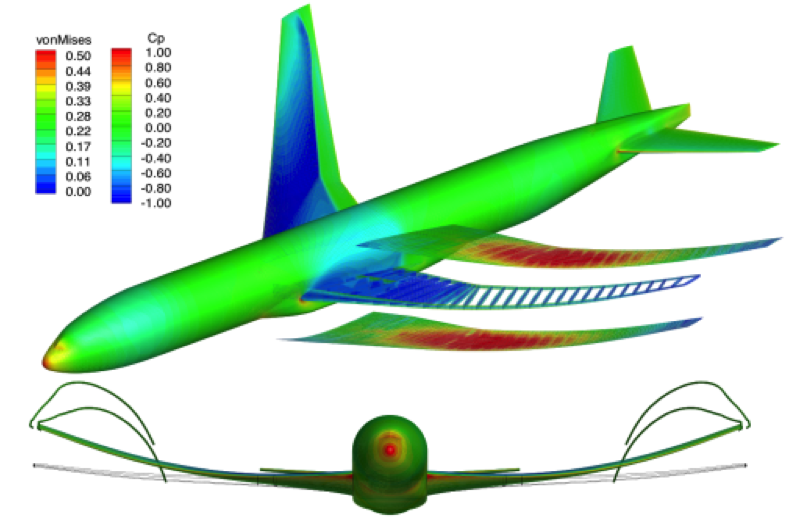
\includegraphics[clip,width=0.65\columnwidth]{./figs/chap1_intro/1_as.png}\label{fig:A}  %
} \\
\subfloat[Topology Optimization~\cite{topo_opt}]{ %
  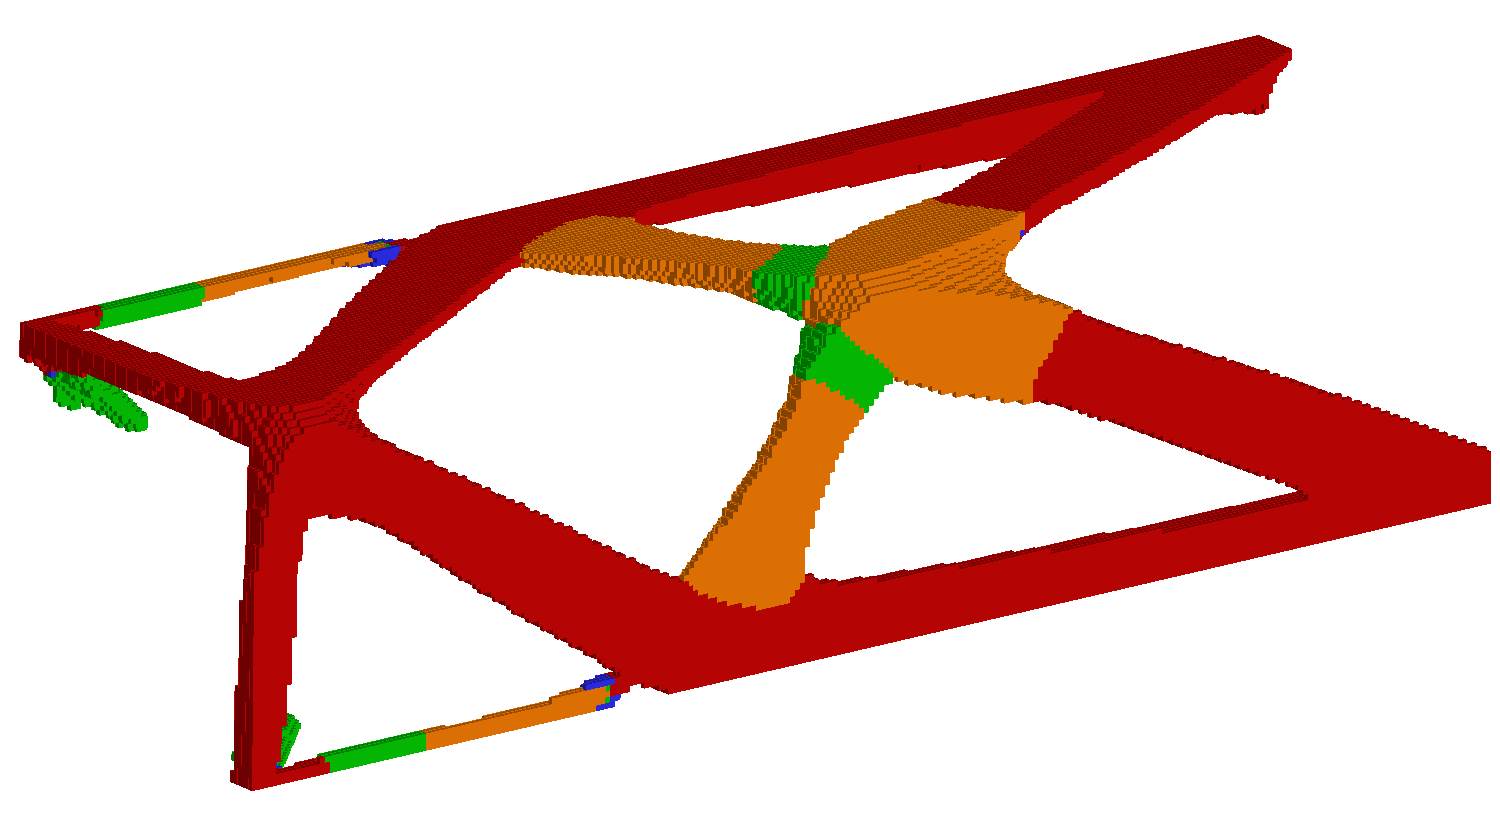
\includegraphics[clip,width=0.65\columnwidth]{./figs/chap1_intro/1_topo.png}\label{fig:B}
}
\caption{Large-Scale PDE-constrained Optimization}
\label{fig:1_mot}
\end{figure}

In such applications, an optimization library is coupled with PDE solvers. The optimizer will ask for the function values and gradients of the objective and constraints, which entail the solutions of the PDE solvers and gradient solvers. Figure~\ref{fig:outflow} illustrates the schematic diagram of the optimization process.   

 \begin{figure}[H]
  \centering
  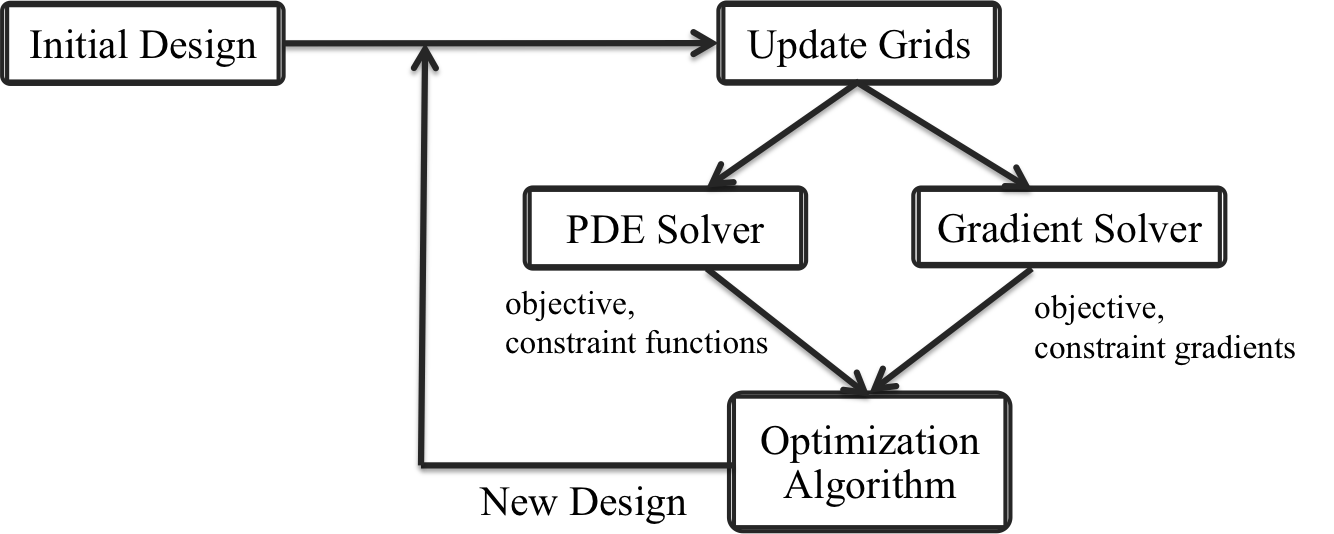
\includegraphics[clip, width=0.8\columnwidth]{./figs/chap1_intro/1_optFlow.png}%  
  \caption{Schematic Process of PDE-constrained Optimization\label{fig:outflow}}
\end{figure}

The difficulty in PDE-constrained optimization is that the PDE solution, also named the state solution, is a sub-problem of the optimization problem, and is a complicated topic itself. During the optimization process, the optimizer will ask for the PDE solution many times for the state variables at different design points; in addition to that, the optimizer calls the gradient solver to compute the gradients of the objective and constraints. 
However, in large-scale engineering, the PDE solve and the gradient evaluation can be very expensive even with the advancement in modern computer power. Moreover, storage of the necessary matrices can impose a heavy burden on computational resources.    

\section{Conventional Optimization Algorithms}
Conventional gradient-based optimization algorithms~\cite{Nocedal2006NO, Byrd:1999:IPA:588897.589167,gill:2002} have been used extensively in PDE-constrained optimizations, particularly for problems with not so many state-based constraints. They use the adjoint methods~\cite{pironneau:1974, jameson:1988, reuther:1996, Jameson03aerodynamicshape, Mader06adjoint:an,  Lyu2013b, hicken:aiaa2010}  
to compute the total objective gradient and the constraint Jacobians. The cost of an adjoint solution is independent of the number of design variables for each objective or constraint. 
To name a few examples, \cite{2015lyu_crm} and \cite{kenway:2014} use SNOPT (Sparse Nonlinear OPTimizer) \cite{gill:2002} through the Python interface pyOpt~\cite{Perez:2011:A} for the investigations of the aerodynamic and aerostructural optimization on the Common Research Model based on RANS. Because there are only three aerodynamic objective and constraints, drag, lift, and pitch moment coefficients, they use the adjoint methods to assemble the total gradients and feed them to SNOPT.  Other general purpose optimization algorithms, IPOPT~\cite{Lyu2014f}, Knitro~\cite{Rumpfkeil2009OptimizationbasedMA}, and a sequential quadratic programming method~\cite{Ning09multidisciplinaryconsiderations}, have all been used for aerodynamic design problems.

However, conventional optimization algorithms are not well suited for large-scale PDE-constrained optimization problems due to scalability and convergence issues, especially when there are many state-based constraints. 
On one hand, in the presence of many state-based constraints, assembling the total constraint Jacobians can get prohibitively expensive, as each constraint Jacobian requires the solution of the adjoint equation whose cost is 
equivalent to that of the PDEs governing equation. If the number of constraints is sufficiently large, it will be prohibitively expensive to compute all the total derivatives for optimization as each one entails an adjoint. 

On the other hand, conventional optimization methods store the constraint Jacobians at every major iteration in order to use direct linear algebra methods to solve the linear systems. These matrix-based approaches result in poor scalability performances for conventional methods with ever-increasing problem sizes. Moreover, conventional methods often use limited-memory quasi-Newton to approximate the Hessian of the Lagrangian, which would bring linear asymptotic convergence rates and are not ideal for large-scale optimization problems. 

\section{Full-space, Reduced-space Methods}\label{sec:pde_mot}
In order to efficiently solve PDE-constrained optimization problems, optimization researchers in different PDE fields have been developing in-house algorithms for their own use. There are two categories of methods: Newton-based full-space methods and Newton-based reduced-space methods. To illustrate the two methods mathematically, it is necessary to start from the generic formulations for PDE-constrained optimization problem, which can be stated as 
\begin{equation}\label{eq:gen1}
\begin{aligned}
\underset{x,u}{\text{min}} \quad &f(x, u) &\\
\text{subject to} \quad &  h(x,u) &= 0  \\
 &  g(x,u) &\geq 0  \\
\text{governed by} \quad &  \mathsf{R}(x, u) &= 0, \\
\end{aligned}
\end{equation}
where $x \in \mathbb{R}^n, u \in \mathbb{R}^v$ are the design and state vectors respectively, and $f: \mathbb{R}^n \rightarrow \mathbb{R}, h: \mathbb{R}^n \rightarrow \mathbb{R}^l, g:\mathbb{R}^n \rightarrow \mathbb{R}^m$ are the objective, equality and inequality constraints respectively. We assume that $f$, $h$ and $g$ have continuous second derivatives. $\mathsf{R}(x, u)$ represents the PDE governing equations for the physics system. 

A solution to~\eqref{eq:gen1} must satisfy the first-order necessary optimaltiy conditions~\cite{Nocedal2006NO}.  These conditions are most easily expressed in terms of the Lagrangian, which is the scalar function defined below
\begin{equation}\label{eq:lag}
\mathsf{L}(x, u, \psi, s, \lambda_h, \lambda_g) = f(x,u) + \lambda_h^T h(x, u) + \lambda_g^T (g(x,u)-s) + \psi^T \mathsf{R}(x,u),
\end{equation} 
where $s \in \mathbb{R}^m$ are the so-called slack variables,  and $\lambda_h \in  \mathbb{R}^l$,  $\lambda_g \in  \mathbb{R}^m$ are the Lagrangian multiplier vectors for equality and inequality constraints, respectively. 

Using $\mathsf{L}$, the first-order necessary, or the \textit{Karush-Kuhn-Tucker} (KKT) optimality conditions for \eqref{eq:gen1} can be expressed as
\begin{equation}\label{eq:kktcond}
\begin{aligned}
\nabla_x \mathsf{L} &= \nabla_x f + \lambda_h^T \nabla_x h + \lambda_g^T \nabla_x g + \psi^T \nabla_x\mathsf{R} = 0, \\
\nabla_u \mathsf{L} &= \nabla_u f + \lambda_h^T \nabla_u h + \lambda_g^T \nabla_u g + \psi^T \nabla_u\mathsf{R} = 0, \\
\nabla_{\psi} \mathsf{L} &= \mathsf{R} = 0, \\
\nabla_{\lambda_h} \mathsf{L} &= h = 0, \\
\nabla_{\lambda_g} \mathsf{L} &= g - s = 0, \\
-\mathsf{S} \mathsf{\Lambda}_g e &= 0,\\
s \geq 0, &\quad \lambda_g \leq 0. \\
\end{aligned}
\end{equation}


%the solution of an $v\times v$ linear system, \ie a discretized PDE.  For example, the total derivative of the $i$th constraint $g_i$ in \eqref{eq:gen1} is given by
%\begin{align}
%\frac{d}{dx}\left(g_i\right) &= \frac{\partial}{\partial x}\left(g_i\right) + \psi ^T \left[ \frac{\partial}{\partial x}\mathsf{F} \right] \\
%\intertext{where $\psi \in \mathbb{R}^v$ is the adjoint which is governed by the discretized PDE,}
%\left[ \frac{\partial}{\partial u}\mathsf{F} \right]^T \psi &= - \frac{\partial}{\partial u}\left(g_i\right) 
%\end{align}
%The computational cost of solving the adjoint equation is equivalent to that of the PDEs governing equation. Clearly, if the number of constraints $m$ is sufficiently large, it will be prohibitively expensive to compute all the total derivatives for optimization as each one entails an adjoint. 


In the context of PDE-constraints, the nonlinear system of equations \eqref{eq:kktcond} can be solved in either the full space or the reduced space.  Full-space methods~\cite{DBLP:journals/siamsc/BirosG05,DBLP:journals/siamsc/BirosG05a,haber:2001} solve all the unknowns in \eqref{eq:kktcond} simultaneously. This results in a large algebraic system consisting of more than double the number of PDE state variables (due to the adjoint).  In addition, if Newton's method is used to solve~\eqref{eq:kktcond}, the resulting linear systems are highly sparse, indefinite, and ill-conditioned. An advantage of the full-space approach is that, 
during the intermediate optimization iterations, the PDE state equation, $\mathsf{R} =0$, and adjoint equation, $\nabla_u \mathsf{L} = 0$, do not need to be solved exactly. This avoids the computational expense of tightly converging the PDE and adjoint equation residuals; however, this is also a potential disadvantage in practical engineering problems, because, if the optimization fails to converge, the intermediate solution may not be feasible with respect to the physics.  Furthermore, for highly nonlinear PDEs, \eg gas dynamics with shocks and boundary layers, practitioners have developed specialized globalization strategies that may be difficult to take advantage of in general-purpose full-space optimization algorithms.  Lastly, no general purpose optimization libraries exist for full-space methods.  

%Newton-based full-space methods possess good scaling, but are complicated to implement as they require intrusion to the PDE solver. 
Reduced-space algorithms for solving~\eqref{eq:kktcond}  
treat the states $u$ and the adjoints $\psi$ as implicit functions of the design variables through $\mathsf{R}(x,u(x)) = 0$, and $\nabla_u \mathsf{L} = 0$. Consequently, the reduced KKT conditions can be formulated as follows:
\begin{equation}\label{eq:opt00x}
 \begin{gathered}
    F(x,s,\lambda_h, \lambda_g) \equiv 
    \begin{bmatrix}
\nabla_x f + \lambda_h^T \nabla_x h + \lambda_g^T \nabla_x g\\
-\mathsf{S} \mathsf{\Lambda}_g e\\
h  \\
g - s 
\end{bmatrix} =0,\\
\text{subject to} \quad s_i \geq 0, \quad \text{and} \quad \lambda_{gi} \leq 0. \\
\end{gathered}
\end{equation}
where the unknowns are $x^T, s^T, \lambda_h^T, \lambda_g^T$, 
and $F :\mathbb{R}^{N} \rightarrow \mathbb{R}^{N}$ is the vector-valued residual
of the KKT conditions, excluding the inequalities on $s$ and $\lambda_g$.  For
notational convenience, we have also introduced $e = [1,1,\ldots,1]^T$ and the diagonal
matrices
\begin{equation*}
  \mathsf{S} = \mydiag\left(s_1,s_2,\ldots,s_m\right),\qquad\text{and}\qquad
  \mathsf{\Lambda}_g = \mydiag\left(\lambda_{g1}, \lambda_{g2}, \ldots, \lambda_{gm}\right).
\end{equation*}

The reduced-space approach to PDE-constrained optimization is attractive for a few reasons.  First, it should be clear that the KKT system~\eqref{eq:opt00x} is much smaller than~\eqref{eq:kktcond}.  Second, reduced-space algorithms are more modular, since they can make direct use of existing PDE primal and adjont solvers.  Of course, the reduced-space approach is not without difficulties.  

The challenges include globalization, which refers to the ability to bypass local minimizers, and nonconvexity handling, which involves bypassing maximizers. The first challenge is addressed in Chapter~\ref{chap:homotopy} and the second in Chapter~\ref{chap:linsys}. 

%\cite{rumpfkeil:2010b} uses a reduced-space Newton algorithm in Knitro to perform steady and unsteady aerodynamic shape optimization, with less computational cost compared with a quasi-Newton method; but the reduced Hessian is computed explicitly. 

\section{Inexact-Newton Methods}
To solve the reduced-space KKT conditions \eqref{eq:opt00x} for PDE-constrained optimization 
problems, a popular alternative to using conventional (matrix-based) optimization algorithms or
constraint aggregation is to apply inexact-Newton methods~\cite{dembo:1982},
also know as truncated-Newton methods in the optimization
literature~\cite{nash:2000}.  

With the exception of the bounds on $s$ and $\lambda_g$, the KKT conditions
\eqref{eq:opt00x} form a set of nonlinear algebraic equations, $F(q)=0$, 
where $q \equiv (x^T, s^T,
\lambda_h^T, \lambda_g^T) \in \mathbb{R}^{N}$ is a vector of all the unknowns.
These equations can be solved, in principle, using Newton iterations of the form
\begin{equation}
(\nabla_q F) \Delta q^{(k)} = -F(q^{(k)}), \label{eq:Newton}
\end{equation}
where $q^{(k)}$ is the solution at the $k$th iteration and $\Delta q^{(k)} =
q^{(k+1)} - q ^{(k)}$ is the solution update.  Solving~\eqref{eq:Newton} exactly
can be inefficient during early Newton iterates when the linear model is not a
good approximation to $F(q)=0$.  Instead, truncated- and inexact-Newton methods
find approximate solutions to \eqref{eq:Newton} that, for example, satisfy the
inexact-Newton condition
\begin{equation}
  \left\| (\nabla_q F) \Delta q^{(k)} + F(q^{(k)}) \right\| \leq \eta_k \left\| F(q^{(k)}) \right\|, \label{eq:inexact_Newton}
\end{equation}
for some parameter $\eta_k \in (0,1)$.


There has been considerable success applying inexact-Newton methods to
unconstrained optimization problems; see \cite{nash:2000} and the references
therein.  On the other hand, inexact-Newton methods for general (nonconvex)
constrained problems are much less common.  Some notable exceptions include the
efforts by Byrd and colleagues~\cite{byrd:2008, byrd:2010} and by Heinkenschloss
and Ridzal~\cite{heinkenschloss:2014}; however, these algorithms make
assumptions regarding the structure of the problem that favor full-space
formulations, and our experience applying them to reduced-space PDE-constrainted
optimization has been disappointing.

Applying Newton's method to \eqref{eq:opt00x}, the KKT system, also called primal-dual system is obtained:
\begin{equation}\label{eq:kkt0}
\begin{bmatrix} \nabla_{xx} \mathsf{L} & 0 & \nabla_x h^T  & \nabla_x g^T  \\
    0 & -\mathsf{\Lambda}_g & 0 & -\mathsf{S} \\
     \nabla_x h & 0 & 0 & 0 \\
    \nabla_x g & -\mathsf{I} & 0 & 0 
    \end{bmatrix}
    \begin{bmatrix} p_x \\ p_s \\ p_h \\ p_g \end{bmatrix}
    = - \begin{bmatrix} \nabla_x \mathsf{L} \\ -\mathsf{S} \Lambda_g e \\ h \\ g - s \end{bmatrix}
\end{equation}
where $\mathsf{L}$ the Lagrangian is defined in \eqref{eq:lag}, $\mathsf{S}$ and $\mathsf{\Lambda}_g$ are as defined previously. 

NK method solves \eqref{eq:kkt0} using Krylov method, so it only need the matrix-vector product of the system matrix. The products are formed in a matrix-free way by solving two second-adjoint systems, for details, see~\cite{hicken:inexact2014, dener:idf2017} and the references therein.  However, while NK methods can avoid the cost associated with forming the explicit constraint Jacobian, the extension to inequality constraints faces several significant challenges. First, active-set and interior-point algorithms that make use of an explicit basis for the null space of the constraint Jacobian cannot be used, because such a basis requires the Jacobian to be explicitly available.  Second, the primal-dual saddle-point system raised in optimization is indefinite and ill-conditioned, making it difficult for iterative Krylov methods to converge to a sufficient tolerance, hurting the convergence rate of Newton's method. Third, dealing with nonconvex Hessian of the Lagrangian in the null space of the constraint Jacobian is also a non-trivial task. 


%The solution to the optimization problem \eqref{eq:opt00x} is a saddle point for the Lagrangian \eqref{eq:lag}, as the optimal design point minimizes the Lagrangian, while the optimal multipliers maximizes the Lagrangian ~\cite{benzi2005numerical}. 
%Note that the matrix in  \eqref{eq:kkt0} is nonsymmetric \footnote{By using a scaled slack block, $\tilde{p_s} = \mathsf{S}^{-1}e p_s $,  the system \eqref{eq:kkt0} can be turned into a symmetric one. We adopt the nonsymmetric version, as we think the preconditioner for this form has better numerical properties, see the section on preconditioner later}. 


%%%%%%%
%Therefore, the resulted KKT system for the reduced-space method is much smaller, and it can make use of existing PDE solvers and adjoint solvers, maintaining modularity. 
Prior to this work, reduced-space methods have been successfully implemented in unconstrained problems and IDF problems. The unconstrained version of \eqref{eq:opt00x} can be solved efficiently using a Newton-Krylov (NK) algorithm applied to the first-order optimality conditions; see, for example, \cite{akcelik:2006, Heinkenschloss:1999:IOA, hinze2010optimization,borzi:2011}. NK optimization algorithms have also shown promise for equality-constrained optimization in the reduced space, because they do not require the constraint Jacobian to be form explicitly and, thus, avoid the scaling issue described earlier.  For instance, \cite{dener:idf2017} applied a matrix-free NK algorithm to a class of equality-constrained optimization problems that arise in multidisciplinary design optimization and would otherwise be intractable with conventional matrix-based algorithms.

%%%%%%%

\section{Challenges in Using Matrix-free Newton-Krylov Methods}
Motivated by its success in the unconstrained and equality-constrained cases, this thesis aims to extend the Newton Krylov methodology to more general, inequality constrained problems, to solve \eqref{eq:opt00x}. 
The goal encounters several challenges listed below, and in doing so represents 
several separate objectives. 

%The objective of this thesis is to develop an efficient inexact-Newton algorithm that is
%suitable for reduced-space PDE-constrained optimization problems of the
%form~\eqref{eq:gen1}.  


\begin{description}
\item[Nonconvexity:] The system $F(q) =0$ does not distinguish between different
  types of stationary points, so a basic Newton's method may converge to local
  maximizers or saddle points.  Conventional optimization algorithms often
  project onto the null-space of the (active) constraint Jacobian to detect
  directions of negative curvature and avoid undesirable stationary points, but
  the null-space is not explicitly available for matrix-free inexact-Newton
  methods.
\item[Preconditioning:] The number of iterations necessary to satisfy the
  inexact Newton condition \eqref{eq:inexact_Newton} using, for example, a
  Krylov method is closely related to the condition number of the system.
  Unfortunately, it is well known that the primal-dual, or KKT, matrix $\nabla_q
  F$ is indefinite and highly ill-conditioned.  A preconditioner is needed that
  is inexpensive to form, factor, and store.  A general-purpose, inexpensive
  preconditioner is especially difficult to find in the reduced-space context,
  since approximations to $\nabla_q F$ are not readily available as they are in
  the full-space.
\end{description}


\section{Thesis Contributions}
This thesis intends to address these challenges by proposing a scalable optimization algorithm especially intended for large-scale PDE-constrained design problems. 
The approach to addressing globalization is to introduce a homotopy map that
implicitly defines a solution curve that connects the solution to an easy
problem to the solution of the desired problem.  Then a
predictor-corrector algorithm is proposed to follow the curve from the easy to the desired
solution.  %A related globalization is used in \cite{Perez2009homotopy} in the
%context of a trust-region managed sequential approximate optimization.  


To address the conditioning of the KKT matrix, a low-rank approximation of 
the Schur complement of the KKT system is proposed. The low-rank approximation 
is computed by using Lanczos method which only involves matrix-vector products of the Schur 
complement. The matrix-vector products are obtained using approximate state and adjoint solutions. 



%In this work, we present a general reduced-space Newton-Krylov optimization algorithm, which is part of the matrix-free optimization package Kona~\cite{dener:scitech2016}, for PDE-constrained optimization problems. It possesses good algorithmic scaling property as it approximates Hessian vector products through second adjoint solves. In addition, a Lanczos based preconditioner 
%is presented to accelerate the convergence of the iterative linear solvers.  



\section{Thesis Outline}
The following contents are organized as follows: 
\begin{itemize}

\item Chapter~\ref{chap:homotopy} reviews the homotopy-based globalization and the homotopy map adopted in this work. Then it describes the predictor-corrector path-following algorithm that traces the homotopy zero curve using Newton-Krylov method. To verify the proposed globalized algorithm, a Sphere problem with a linear objective and a quadratic inequality constraint is tested. Then a synthetic indefinite problem is used to examine the algorithm's ability to bypass local maximum points. 

\item Chapter~\ref{chap:linsys} is focused on describing the proposed matrix-free preconditioner, firstly for solving inequality constrained problems, then for solving problems with both equality and inequality constraints. A synthetic quadratic problem with linear inequality constraints is used to investigate the effectiveness of the inequality preconditioner and the scalability performance of the algorithm. 

\item Chapter~\ref{chap:tests} begins with introducing the optimization environment Kona and a state-of-the-art optimization algorithm SNOPT against which comparisons will be made.  The new algorithm and the preconditioners are tested on three problems: firstly on a subset of the CUTEr problems, secondly on a mass minimization stress-constrained structural problem, and lastly on an aerodynamic shape optimization problem. 
 
\item Chapter~\ref{chap:con} provides conclusions and some suggestions for future works. 
\end{itemize}


%For PDE-constrained optimization problems, when there are many state-based constraints, assembling the total constraint Jacobian is very expensive as it demands an adjoint solve for each state-based constraint. Additionally, general optimization algorithms store the constraint Jacobians at each design point, which puts a heavy memory load on the computer. Therefore, most general optimization algorithms possess poor scaling qualities.  
%The first aerodynamic optimization was done in \cite{hicks:1974} by using finite-difference approximations to calculate the gradients. The cost of computing the gradients using finite-difference methods increases drastically as the design dimension increases. The adjoint methods have greatly propelled the advancement of research in aerodynamic shape optimization field. Adjoint methods address the dimensionality issue of finite-differences with a cost independent of the number of design variables. \cite{pironneau:1974} developed the adjoint method for Stokes equations and the incompressible Euler equations, and used the adjoints to optimize airfoil profiles. \cite{reuther:1996} used an adjoint algorithm based on Euler to optimize a complete aircraft configurations.  \cite{jameson:1988} derived the adjoint equations for inviscid compressible Navier-Stokes equations, making it possible to do transonic aerodynamic optimizations.  The discrete adjoint method is more preferred in aerospace optimization as the sensitivities are exact to the discretized objective function~\cite{frank:1992}. \cite{Mader06adjoint:an} derived a discrete adjoint method for Euler equations using automatic differentiation. \cite{Lyu2013b} extended the previous adjoint implementation to 
%Reynolds-averaged Navier-Stokes (RANS) equations and effectively applied it to high-fidelity optimization. \cite{hicken:aiaa2010} developed similar methods for non-planar wings high-fidelity aerodynamic optimization. 



%The simulation problem solves the PDEs for state variables, e.g. the pressure distribution along the surface mesh node points on the wing in Figure~\ref{fig:A}, and the displacement distribution among the solid mesh node points in Figure~\ref{fig:B}, at certain design variables. 

%The performance of the physics system is evaluated in the form of objective function bounded by certain constraints, while the objective and the constraints depend on both the state variables and the design variables. The optimizer will choose a design point, inquire the PDE solver for state variables, and compute the functional values and the gradients of the objective and constraints at that point. 

%The optimizer will process all the information and yield a better design point using mathematical algorithms. The process is repeated until certain criteria is met for optimality.  



% \section{Optimization Algorithms}

%Conventionally, solving general constrained optimization problems without PDE constraints involves forming the Lagrangian, and finding the minimization point of the Lagrangian, which is equivalent to solving the first-order optimality conditions or the KKT conditions. Prevalent sequential quadratic programming methods or newton-type methods for solving a system of equations would further break it down to solving a series of systems of linearized equations, also called the Karush-Kuhn-Tucker (KKT) system. The KKT matrix contains the Hessian of the Lagrangian, which is often approximated using quasi-Newton method, and the total constraint Jacobians, which is straightforward to compute using automatic differentiation or complex step methods. Conventional matrix-based optimization algorithms would use direct factorization methods to solve the KKT system.    

%The kernel of reduced-space Newton-Krylov methods for PDE-constrained optimization solves a series of linear systems, which are saddle point systems, but much smaller than the saddle-point system raised in full-space methods.  Because the solution to the optimization problem \eqref{eq:opt00x} is a saddle point for the Lagrangian \eqref{eq:lag} in that the optimal design point minimizes the Lagrangian, while the optimal multipliers maximizes the Lagrangian ~\cite{benzi2005numerical}.  


%%%%%%%%%%%%

% a popular large-scale matrix-based active -set augmented-Lagrangian optimization method SNOPT.  

%\begin{equation}\label{eq:saddle}
%\mathsf{A} = \begin{bmatrix}
%A & B \\
%C & D
%\end{bmatrix}
%\end{equation}
%One type of Schur complement can be obtained by performing the following LDU decomposition 
%\begin{equation}\label{eq:saddle:ldu}
%\mathsf{A} = \begin{bmatrix}
%A & B \\
%C & D
%\end{bmatrix} = 
%\begin{bmatrix}
%I_p & BD^{-1} \\
%0 & I_q
%\end{bmatrix}
%\begin{bmatrix}
%A-BD^{-1}C  & 0 \\
%0  & D 
%\end{bmatrix}
%\begin{bmatrix}
%I_p  & 0 \\
%D^{-1}C  & I_q 
%\end{bmatrix}
%\end{equation}

% which is indefinite, poor spectral properties (ill-conditioned) 
% Direct solvers, however, are still the preferred method in optimization and other areas. Furthermore, direct methods are often used in the solution of subproblems, for example as part of a preconditioner solve.
%The preconditioners developed here are tailored for PDE-constrained optimization problem. 
% matrix-vector products with A can be performed efficiently
% approximate its action on a vector with (nearly) linear complexity,
% the convergence of the iterates to the optimal solution of problem
% gain efficient, save on storage
%words from the paper ~\cite{benzi2005numerical} Benzi block preconditioners, 
% As the iterates approaches the solution,  the entries in A tend to zero, or infinity, KKT matrix ill-conditioned
% the norm of the inverse Schur complement goes to infinity

% Schur complement reduction 
% null space methods, the null space of the constraint Jacobian, the column of Z span the null space of constraint Jacobian
% popular in optimization, projection of the problem onto the constraint set; 

 
%%% Local Variables: 
%%% mode: latex
%%% TeX-master: t
%%% End: 

%The formula \eqref{eq:kkt0} takes the same form as the classical interior point method in Chapter 19 in Nocedal's book \cite{Nocedal2006NO}, which will be reviewed below. 

%\section{Review on Interior Point Method  }
%The difficulty in extending the Newton Krylov methods to handle inequality constraints, to solve \eqref{eq:opt00x} lies in the nonlinear complementarity condition: for each inequality constraint, either the slack or Lagrangian multiplier is strictly zero if we assume strict complementarity is satisfied at the solution. The slack has to be non-negative to guarantee feasibility of the inequality constraints, and the multipliers has to be non-positive in respect to the property of a local minimization point following the formula convention. For inequality constraints that are active at the solution, slack variable is zero and the multiplier is negative, while for inactive inequality constraints, slack variable is positive and the multiplier is negative. Therefore, the complementarity condition, in combined with the sign requirement on slack and multipliers, contains information on optimal active set of the inequality constraints at the solution.   
%
%Currently there are two most powerful algorithms for general nonlinear constrained problems: active-set SQP methods and interior point methods \cite{Nocedal2006NO}. Determining the inequality constraint sets that are active at the solution is the main challenge facing active-set methods. Especially when the number of inequality constraints is large, the method may need many iterations to locate the active-set of inequality constraints. While for interior point methods, there are two varieties based on globalization strategies: Newton-Lagrangian line-search and trust-region SQP on the barrier problems. The former is more for illustration purpose, and the latter is actually implemented in practical optimization software libraries IPOPT \cite{W�chter2006}, and KNITRO \cite{Byrd:1999:IPA:588897.589167}. 
%
%The trust-region SQP method builds a quadratic model on the barrier formulation, employs direct linear algebra, uses explicit constraint Jacobians to first compute the multipliers that deliver minimum linearized constraint violations, then compute the design and slack update steps that minimize the quadratic model. In both subproblems, a trust region bound is imposed on the design and slack components, with the slack variable scaled properly to prevent it away from the nonnegative bound. A proper merit function mimic the quadratic objective function is used to estimate the quality of the steps and control the trust-region radius for next iteration. 
%
%To handle nonlinearities and nonconvexities, regularization terms can be added to the Hessian block and the equality constraint Jacobian on the diagonal of the KKT matrix. The proper amount of regularization is computed at each iteration by trial and error such that the inertia of the regularized KKT matrix is $(n+m, l+m, 0)$, under which condition the total Hessian block of design and slack will be positive definite on the null space of the combined constraint matrix, therefore the resulted Newton step will be a guaranteed descent direction for a large class of merit functions. 
%
%Using the proper barrier parameter $\mu$ updating strategy is crucial to the performance of interior point methods: A slowly decreasing $\mu$ will result in large number of outer iterations, making the algorithm less efficient. While a quickly decreasing $\mu$ may make some slack or inequality multipliers approach zero prematurely, hurting the convergence. Some simple implementations of interior point methods use a constant fraction updating scheme, while some chooses the fraction value based on the recent iterations' progress towards the solution. Making the fraction value close to zero near the solution can yield a superlinear convergence rate. More robust strategies update $\mu$ based on the progress of the current complementarity products. Predictor strategy first calculates a predictor direction by setting $\mu=0$, then calculates the tentative complementarity product along this direction using the step size from fraction to boundary rule. The updating fraction value is based on the ratio of this tentative and current complementarity product. 
%
%
%The former Newton-Lagrangian line-search method solves a perturbed KKT system at each homotopy parameter, also called the barrier parameter $\mu$:
%
%\begin{equation}\label{eq:kkt1}
%\begin{aligned}
%\nabla f(x) + \lambda_h^T \nabla h(x) + \lambda_g^T \nabla g(x) &= 0 \\
%-\mathsf{S} \Lambda_g - \mu e &= 0\\
%h(x) &= 0 \\
%g(x) - s &= 0 \\
%s \geq 0, \quad &\lambda_g \leq 0 \\
%\end{aligned}
%\end{equation}
%The barrier parameter $\mu$, is a sequence of strictly positive numbers and converges to zero. The perturbed KKT system \ref{eq:kkt1} is solved for each $\mu$, and the solution trajectory converges to the KKT point of the original problem in the limit.  
%
%Newton's method is used to solve \ref{eq:kkt1} for each $\mu$, where each Newton step is as follows:
%\begin{equation}
%\begin{bmatrix} \mathsf{W} & 0 & \mathsf{A}_{h}^T & \mathsf{A}_{g}^T \\
%    0 & -\Lambda_g & 0 & -\mathsf{S} \\
%    \mathsf{A}_{h} & 0 & 0 & 0 \\
%    \mathsf{A}_{g} & -\mathsf{I} & 0 & 0 
%    \end{bmatrix}
%    \begin{bmatrix} p_x \\ p_s \\ p_h \\ p_g \end{bmatrix}
%    = -\begin{bmatrix} \nabla_x \mathsf{L} \\ -\mathsf{S} \Lambda_g - \mu e  \\ h(x) \\ g(x) - s \end{bmatrix}
%\end{equation}
%After the Newton step direction is computed, fraction to the boundary rule is applied to determine the maximum allowable step size to keep the slack and inequality multipliers away from the 0 bound. Then a backtracking line search is performed to find the step length that delivers sufficient decrease in the merit function or accepted by the filter. The barrier parameter is then updated for the next iteration. 
%
%There are potential drawbacks when using interior point methods for PDE-constrained optimization. For instance, to ensure progress towards global minimum, either trust-region or line-search globalization techniques have to be implemented. The former judges the quality of a computed step by calculating the merit function value and adjust the trust-region radius accordingly, while the latter computes the step-length along a step direction that satisfies the Wolfe condition. In either case, extra computation is needed. Dealing with nonconvex Hessian of the Lagrangian in the null space of the constraint Jacobian is also a non-trivial task; possible solutions include adding a proper regularization term to enforce a positive definite Hessian, see \cite{hicken:flecs2014} and Algorithm B.1 \cite{Nocedal2006NO}. Moreover, the saddle-point matrix raised in optimization is indefinite and ill-conditioned, making it difficult for iterative Krylov methods to converge. 


